The infrastructure implemented for the experiments presented below is open
source and available online at \cite{sources}. The implementation is based on
TensorFlow \cite{abadi2015}, which is an efficient, flexible, and highly
scalable machine-learning library supported by all the major platforms including
the mobile ones.

The experiments are conducted on a \up{GNU}/Linux machine equipped with 16
\up{CPU}s Intel Xeon \up{E5520} 2.27~GHz, 24~\up{GB} of \up{RAM}, and an
\up{HDD}. The machine has no modern \up{GPU}s; therefore, the reported results
have an immerse room for improvement, which concerns not only timing but
potentially accuracy as well due to more extensive training.

\subsection{Data Processing}
Recall that we work with the Google cluster-usage traces \cite{reiss2011}; see
the introduction in \sref{data}. In the experiments, we focus on one particular
resource ($d = 1$), which is the \up{CPU} usage of the tasks run in the cluster.
The resource-usage table contains two apposite columns: the average and maximal
CPU usage over five-minute intervals; we extract the former.

The grouping and indexing steps of the data-processing pipeline described in
\sref{grouping} and \sref{indexing}, respectively, take approximately 60 hours
or 2--3 days (no parallelism). Most of this time is spent converting \up{CSV}
into SQLite, which can be avoided by working with \up{CSV} directly. However,
SQLite provides a convenient way for working with the data. Moreover, since
these operations have to be done only once, their computational cost can be
safely considered negligible.

\begin{figure}[t]
  \centering
  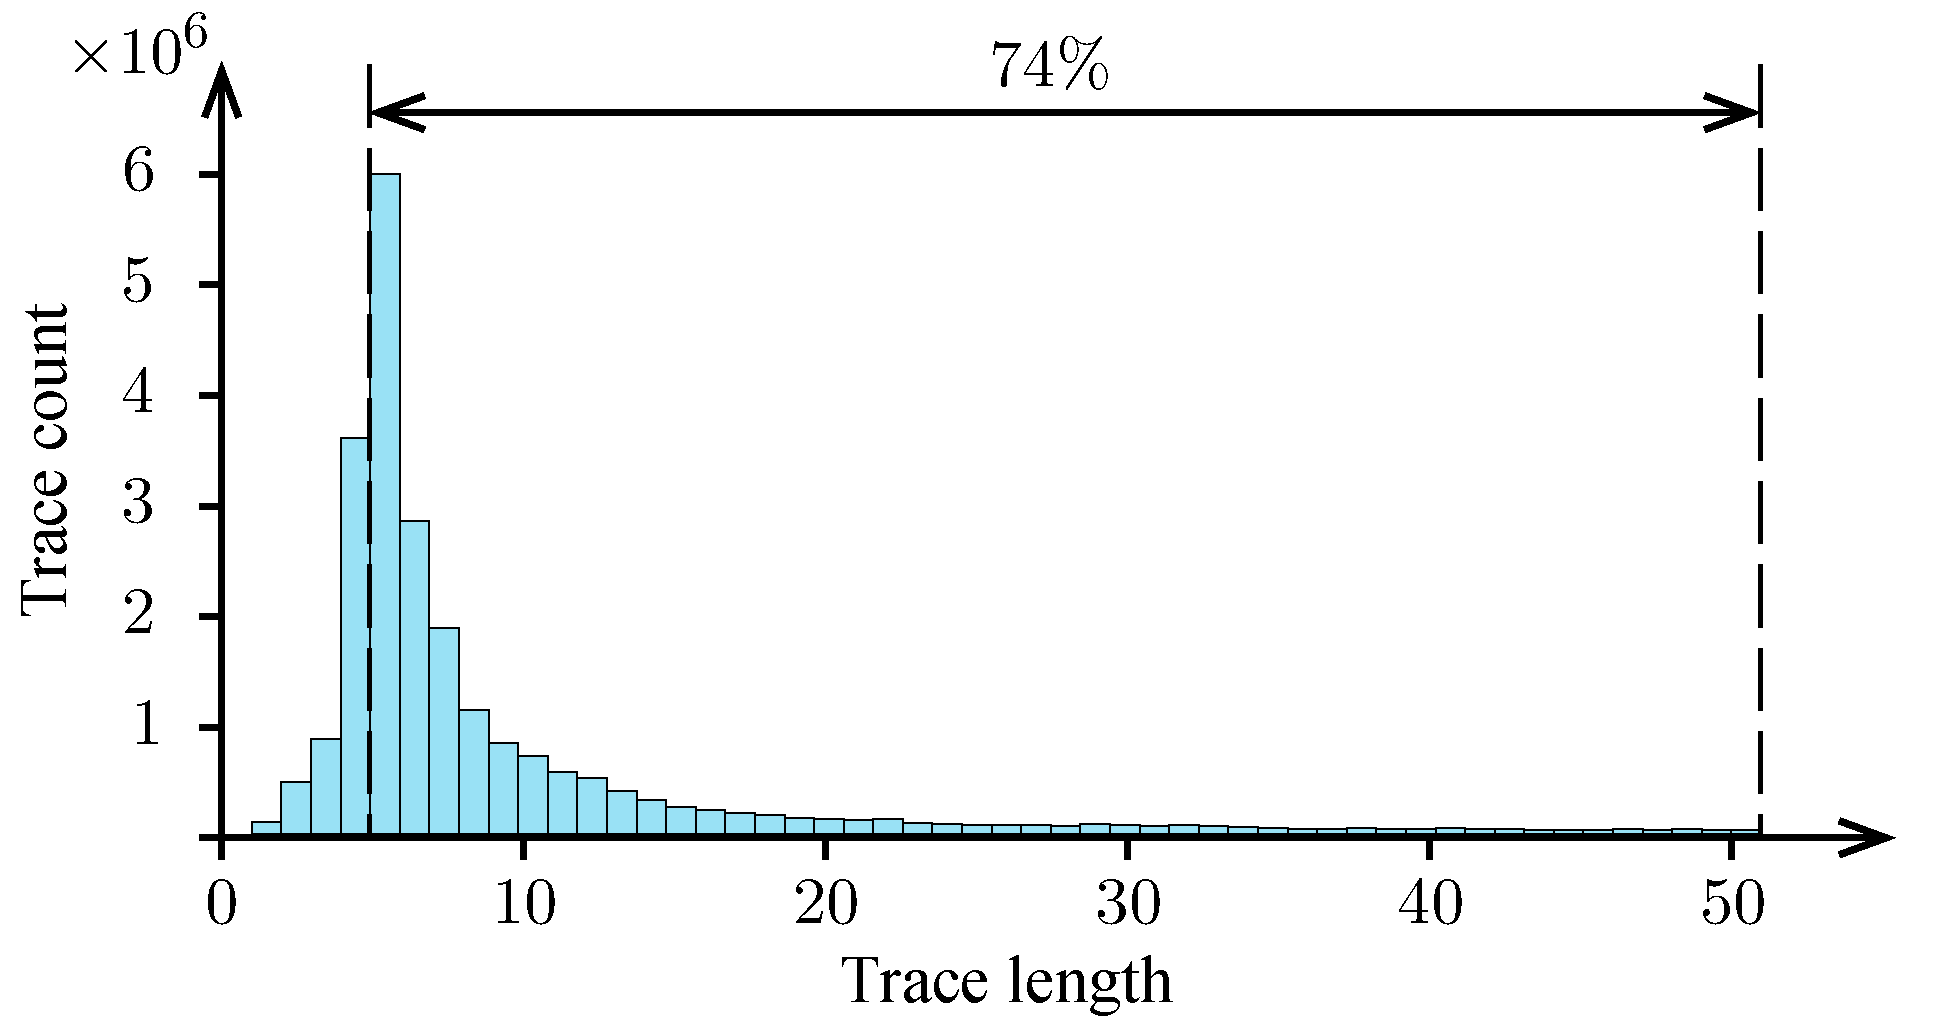
\includegraphics[width=1.0\columnwidth]{include/assets/figures/traces.pdf}
  \vspace{-1.5em}
  \caption{
    The histogram of the lengths of the resource-usage traces. It has been
    truncated on the right in order to show the bulk of the distribution better.
  }
  \vspace{-1.5em}
  \flab{traces}
\end{figure}

Regarding the selection stage delineated in \sref{selection}, we filter those
traces that contain 5--50 data points; thus, $l_i \in [5, 50]$ in \eref{trace}.
It can be seen in \fref{traces}, which shows a truncated histogram of the
traces' lengths, that such traces constitute around 74\% of the total number of
traces (around 18 out of 24 million).

We experiment with a subset of two million random traces, which is around 11\%
of the 5--50 resource-usage traces; hence, $n = 2 \times 10^6$ in \eref{traces}.
The data sets $X_1$, $X_2$, and $X_3$ constitute 70\%, 10\%, and 20\% of $X$,
respectively. Fetching and storing on disk these many traces take less than
three hours. Recall that this operation has to be repeated only when the
selection criteria change, which happens rarely in practice.

\subsection{Modeling and Prediction}
The training state (\sref{training}) is configured as follows. Based on
\fref{traces}, 10 buckets are used according to the rule: $l < 6 < 7 < 8 < 9 <
10 < 15 < 20 < 30 < 40 \leq 50$. The batch size $b$ is set to 64. The variant of
gradient descent that we employ for minimizing of the loss function is Adam
\cite{kingma2014}, which is an adaptive algorithm. The algorithm is utilized
with its default settings recommended by the algorithm's authors.

Regarding the validation stage (\sref{validation}), the considered
hyperparameters are the number of cells $c$ (blue boxes in \fref{model}), number
of units per cell $u$ (double circles in \fref{model}), and probability of
dropout $p$. More concretely, we let $c \in \{1, 2, 3, 4, 5\}$, $u \in \{100,
200, 400, 800, 1600\}$, and $p \in \{0.0, 0.1\}$, which yields 50 different
combinations in total. The combinations are explored by means of the Hyperband
algorithm, which is introduced in \sref{validation}, with its default settings.

The above-mentioned exploration, which encompasses both the training and
validation stages, takes around 134 hours or 5--6 days. During this process, we
run up to 8 learning sessions in parallel, which typically keeps all 16
\up{CPU}s busy. It should be noted that, due to the fact that the training,
validation, and testing data have been cached on disk as a result of our
data-processing pipeline described in \sref{data}, individual learning sessions
do not have any overhead in this regard.

\begin{figure}[t]
  \centering
  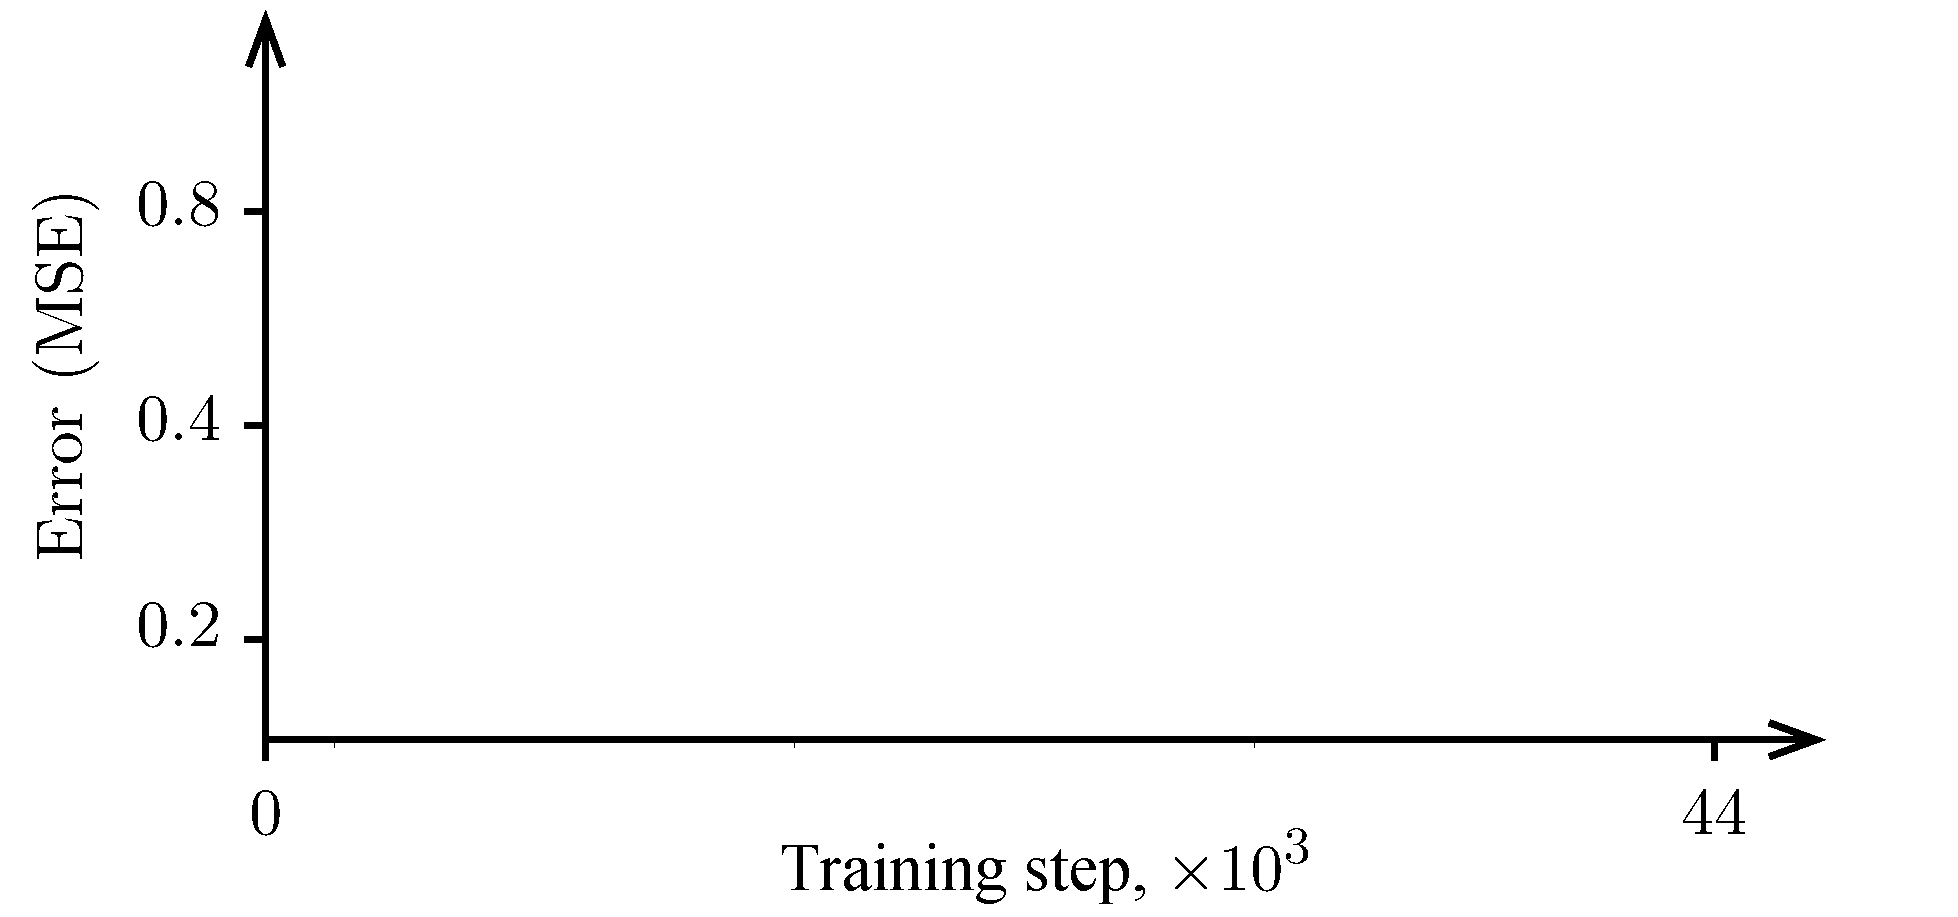
\includegraphics[width=1.0\columnwidth]{include/assets/figures/validation.pdf}
  \caption{
    The error of multiple configurations of hyperparameters with respect to the
    validation set $X_2$ while training using the training set $X_1$.
  }
  \vspace{-1.5em}
  \flab{validation}
\end{figure}

The results of the validation stage can be seen in \fref{validation}, which
shows the mean squared error (\up{MSE}) of different configurations of the
hyperparameters as measured using $X_2$.

After the exploration stage, the best trained model is taken to the testing
stage (\sref{testing}), which is undertaken using $X_3$. At this stage, the
model is extensively assessed by predicting the resource usage of individual
tasks multiple steps ahead at each time step of the testing traces in $X_3$.
In these experiments, we predict four steps ahead ($h = 4$ in \sref{problem}).
This elaborate testing procedures takes around 15 hours to finish.

In order to have a baseline for the accuracy of our resource-usage prediction,
we use a model based on random walk \cite{hastie2009}, which we shall refer to
as the reference. This model assumes that the next value is equal to the current
one plus a optional random offset, which we set to zero for simplicity.

\begin{figure}
  \centering
  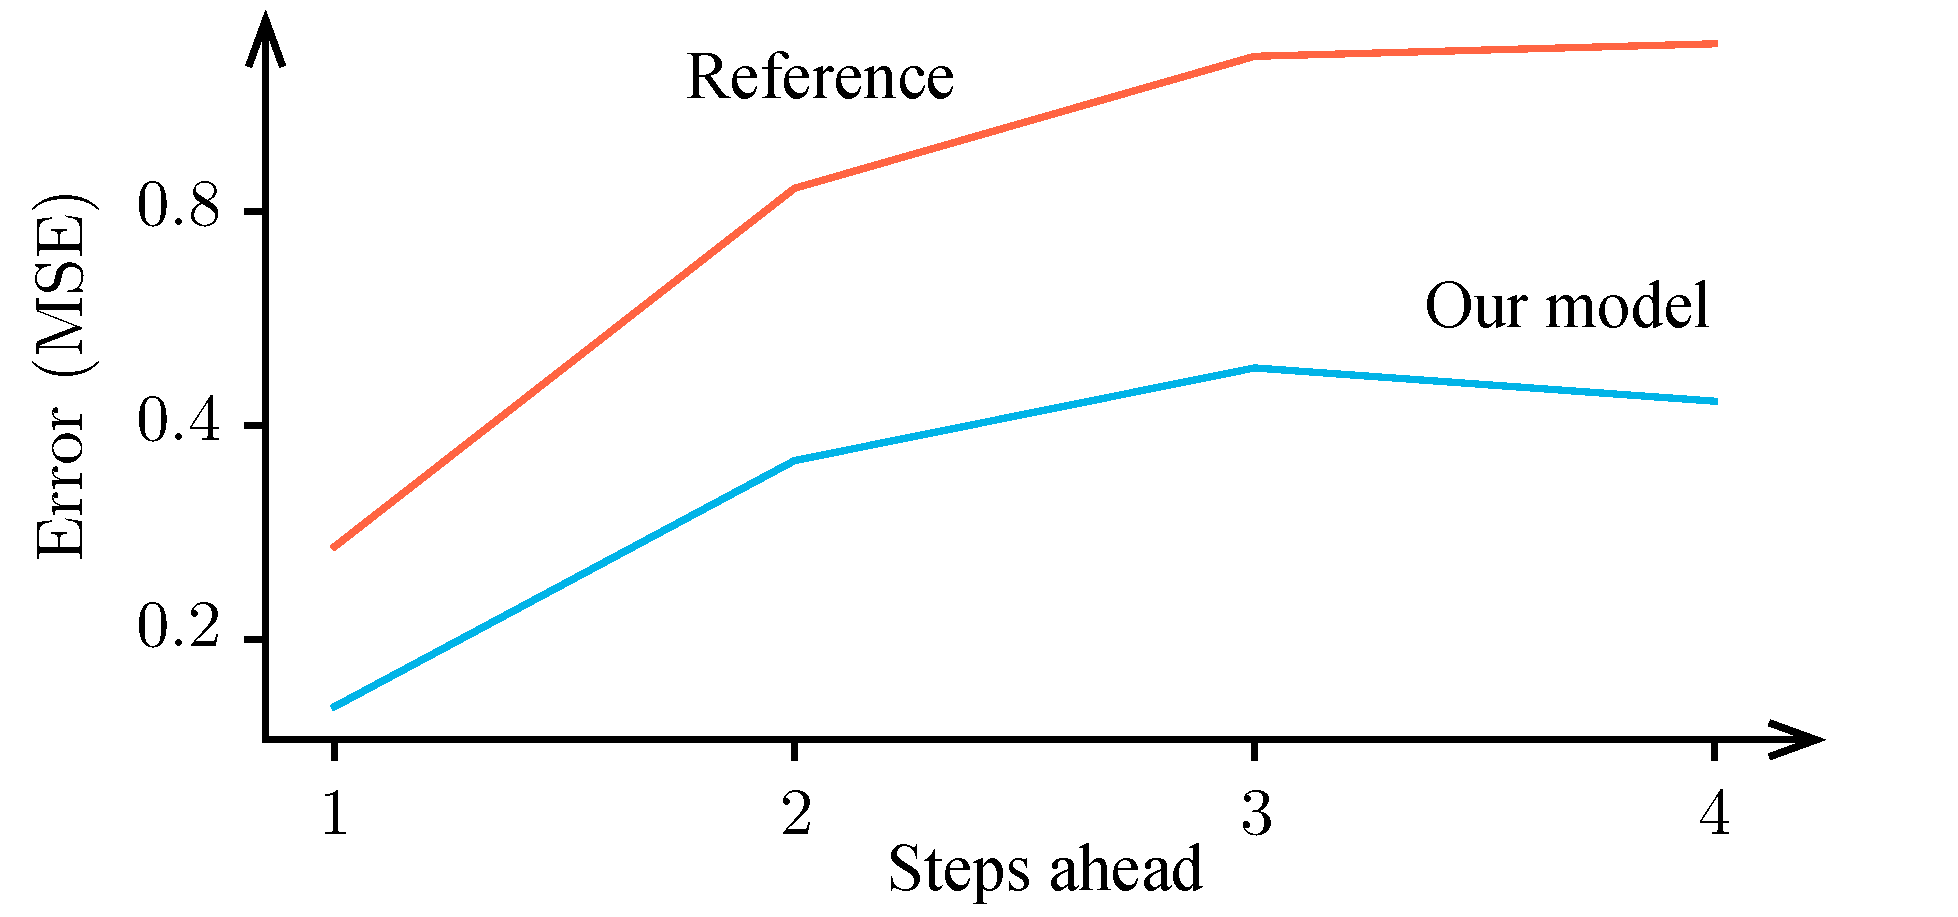
\includegraphics[width=1.0\columnwidth]{include/assets/figures/testing.pdf}
  \vspace{-1.5em}
  \caption{
    Accuracy of predictions up to four steps ahead by our model (blue) and by
    the reference one (red) with respect to the testing set $X_3$.
  }
  \vspace{-1.5em}
  \flab{testing}
\end{figure}

The results of the testing stage can be seen in \fref{testing}, which shows the
\up{MSE} of the chosen model with respect to $X_3$.
